\section{Results and details}\label{sec:results}
In this section, we present execution times for each method depending on angular sampling $S_\theta$ which should result in linear computational complexity. Section \ref{sec:results:sequential} shows times for sequential execution which is then marked as a grey area for comparison. Every chart contains native C++ times. 

\subsection{Sequential}\label{sec:results:sequential}

% MARK: times math
Analyzing benchmark times shown in Figure \ref{plot:sequential} we can see the advantage of Chrome over Firefox being $1.6\times$ faster in the \textit{non-LUT} variant and $2.08\times$ in the \textit{LUT} one. It it worth to notice the optimization in Firefox for the $S_\theta=5$ and subsequent sampling values in the \textit{LUT} variant which could be an object of further research. The performance of server-side environments, Node and Deno, since they are very similar environments, has only insignificant differences, yet still being $(1.50, 1.45)\times$ slower that Chrome for both variants.



\begin{figure}
    \groupBenchmark{
        \plotBenchmark{cpp_theta_SHT_Simple.csv}{cppColor}{{}}
        \addlegendentry{C++}

        \plotBenchmark{js-sequential_theta_SHT_Simple_node.csv}{nodeColor}{{}}
        \addlegendentry{Node}

        \plotBenchmark{js-sequential_theta_SHT_Simple_deno.csv}{denoColor}{{}}
        \addlegendentry{Deno}

        \plotBenchmark{js-sequential_theta_SHT_Simple_Firefox.csv}{firefoxColor}{{}}
        \addlegendentry{Firefox}

        \plotBenchmark{js-sequential_theta_SHT_Simple_Chrome.csv}{chromeColor}{{}}
        \addlegendentry{Chrome}

    } {
        \plotBenchmark{cpp_theta_SHT_Simple_Lookup.csv}{cppColor}{{}}
        \addlegendentry{C++}

        \plotBenchmark{js-sequential_theta_SHT_Simple_Lookup_node.csv}{nodeColor}{{}}
        \addlegendentry{Node}

        \plotBenchmark{js-sequential_theta_SHT_Simple_Lookup_deno.csv}{denoColor}{{}}
        \addlegendentry{Deno}

        \plotBenchmark{js-sequential_theta_SHT_Simple_Lookup_Firefox.csv}{firefoxColor}{{}}
        \addlegendentry{Firefox}

        \plotBenchmark{js-sequential_theta_SHT_Simple_Lookup_Chrome.csv}{chromeColor}{{}}
        \addlegendentry{Chrome}
    } {
        \plotBenchmark{cpp_theta_CHT_Simple.csv}{cppColor}{{}}
        \addlegendentry{C++}

        \plotBenchmark{js-sequential_theta_CHT_Simple_node.csv}{nodeColor}{{}}
        \addlegendentry{Node}

        \plotBenchmark{js-sequential_theta_CHT_Simple_deno.csv}{denoColor}{{}}
        \addlegendentry{Deno}

        \plotBenchmark{js-sequential_theta_CHT_Simple_Firefox.csv}{firefoxColor}{{}}
        \addlegendentry{Firefox}

        \plotBenchmark{js-sequential_theta_CHT_Simple_Chrome.csv}{chromeColor}{{}}
        \addlegendentry{Chrome}
    }
    [3400][850][14]
    \caption{Wyniki pomiarów czasu wydajności dla wykonania sekwencyjnego SHT i CHT.}
    \label{plot:sequential}
\end{figure}


We detected one pixel difference in generated accumulator between variants as shown in Figure \ref{fig:diff:seq_lut} (upper right corner). We implemented lookup table for \textit{LUT} variants using \texttt{Float32Array}. JS internally, without optimizations, represents numbers in double-precision and reduced precision of cached values can have significant impact on detection results.

\begin{figure}
    \begin{subfigure}{0.29\textwidth}
        
\includegraphics[width=\linewidth] {../../packages/js-benchmarks/img/diff_seq_seq_lookup.png}
        \caption{Sequential \textit{LUT}}\label{fig:diff:seq_lut}
    \end{subfigure}\hfill
    \begin{subfigure}{0.29\textwidth}
        
\includegraphics[width=\linewidth] {../../packages/js-benchmarks/img/diff_seq_wasm.png}
        \caption{WASM}\label{fig:diff:wasm}
    \end{subfigure}\hfill
    \begin{subfigure}{0.29\textwidth}
        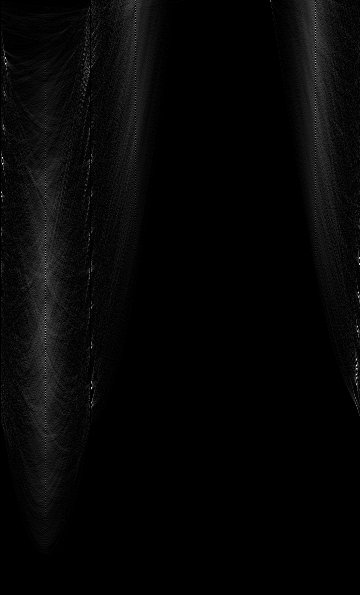
\includegraphics[width=\linewidth] {../../packages/js-benchmarks/img/diff_seq_gpu.png}
        \caption{WebGL}\label{fig:diff:gpu}
    \end{subfigure}
    \caption{Normalized absolute accumulator difference from sequential \textit{non-LUT} variant. Note the two-pixel difference in the upper right corner for Sequential \textit{LUT}.}\label{fig:diff}
\end{figure}


\subsection{Node C++ addon}\label{sec:results:cpp-addon}

C++ addon for Node was built using the same shared library as the C++ version. Thus the difference in performance between native C++ and the addon arise mostly from handling data transfer between C++ -- JS boundary since the data needs to be copied and transformed to corresponding C++ structures. Results are shown in Figure \ref{plot:cpu-addon}.



\begin{figure}
    \groupBenchmark{
        \plotBenchmark{cpp-addon_theta_SHT_Simple_node.csv}{nodeColor}{{}}
        \addlegendentry{Node}

        \seqReference
    } {
        \plotBenchmark{cpp-addon_theta_SHT_Simple_Lookup_node.csv}{nodeColor}{{}}
        \addlegendentry{Node}

        \seqReferenceLookup
    }[1600][650]
    \label{plot:gpu}
    \caption{Node C++ addon SHT execution benchmark results.}
\end{figure}



% MARK: times math
Compilation with optimization of trigonometric functions in \textit{non-LUT} variant allowed to gain more performance ($2.21\times$) than compilation of the \textit{LUT} variant ($1.38\times$) relative to their sequential variants. This case allows us to draw a conclusion that if an algorithm has trigonometric functions and output of which cannot be cached beforehand, the usage of the C++ addon in Node is beneficial.

\subsection{WebAssembly and asm.js}\label{sec:results:asm-wasm}

Benchmark results for asm.js and WASM were shown on figures \ref{plot:asm} and \ref{plot:wasm} respectively. In our case asm.js - a highly optimizable subset of JS instructions, operating only on numeric types and using heap memory - is actually slower in all environments than sequential execution. We suspect that it is caused by the building process. Webpack adds its own module resolution mechanisms that prevent part of the bundle with asm.js code from being recognized and compiled ahead-of-time. Performance flame chart from Chrome DevTools tools shows a lack of \texttt{Compile Code} blocks, unlike any other isolated asm.js sample.

WASM on the other hand improves performance for \textit{non-LUT} variant and has no effect on \textit{LUT} variant besides preventing optimization mentioned in section \ref{sec:results:sequential} in Firefox. Again, it is beneficial to use this method if the output if trigonometric functions cannot be cached.

In our C++ implementation we use single precision floating point variables. This results in accumulator differences shown in Figure \ref{fig:diff:wasm} since WASM distinguishes between \texttt{f32} and \texttt{f64} types.



\begin{figure}[ht]
    \groupBenchmark{
        \plotBenchmark{js-asm_theta_SHT_Simple_node.csv}{nodeColor}{{}}
        \addlegendentry{Node}

        \plotBenchmark{js-asm_theta_SHT_Simple_Firefox.csv}{firefoxColor}{{}}
        \addlegendentry{Firefox}

        \plotBenchmark{js-asm_theta_SHT_Simple_Chrome.csv}{chromeColor}{{}}
        \addlegendentry{Chrome}

        \seqReference
    } {
        \plotBenchmark{js-asm_theta_SHT_Simple_Lookup_node.csv}{nodeColor}{{}}
        \addlegendentry{Node}

        \plotBenchmark{js-asm_theta_SHT_Simple_Lookup_Firefox.csv}{firefoxColor}{{}}
        \addlegendentry{Firefox}

        \plotBenchmark{js-asm_theta_SHT_Simple_Lookup_Chrome.csv}{chromeColor}{{}}
        \addlegendentry{Chrome}

        \seqReferenceLookup
    }{
        \plotBenchmark{js-asm_theta_CHT_Simple_node.csv}{nodeColor}{{}}
        \addlegendentry{Node}

        \plotBenchmark{js-asm_theta_CHT_Simple_Firefox.csv}{firefoxColor}{{}}
        \addlegendentry{Firefox}

        \plotBenchmark{js-asm_theta_CHT_Simple_Chrome.csv}{chromeColor}{{}}
        \addlegendentry{Chrome}

        \seqReferenceCircle
    }[9000][2300][25]
    \caption{Wyniki pomiarów czasu wydajności dla wykonania SHT i CHT z wykorzystaniem kompilacji do asm.js.}
    \label{plot:asm}
\end{figure}


\begin{figure}[h]
    \groupBenchmark{
        \plotBenchmark{js-wasm_theta_SHT_Simple_node.csv}{nodeColor}{{}}
        \addlegendentry{Node}

        \plotBenchmark{js-wasm_theta_SHT_Simple_Firefox.csv}{firefoxColor}{{}}
        \addlegendentry{Firefox}

        \plotBenchmark{js-wasm_theta_SHT_Simple_Chrome.csv}{chromeColor}{{}}
        \addlegendentry{Chrome}

        \seqReference
    } {
        \plotBenchmark{js-wasm_theta_SHT_Simple_Lookup_node.csv}{nodeColor}{{}}
        \addlegendentry{Node}

        \plotBenchmark{js-wasm_theta_SHT_Simple_Lookup_Firefox.csv}{firefoxColor}{{}}
        \addlegendentry{Firefox}

        \plotBenchmark{js-wasm_theta_SHT_Simple_Lookup_Chrome.csv}{chromeColor}{{}}
        \addlegendentry{Chrome}

        \seqReferenceLookup
    } {
        \plotBenchmark{js-wasm_theta_CHT_Simple_node.csv}{nodeColor}{{}}
        \addlegendentry{Node}

        \plotBenchmark{js-wasm_theta_CHT_Simple_Firefox.csv}{firefoxColor}{{}}
        \addlegendentry{Firefox}

        \plotBenchmark{js-wasm_theta_CHT_Simple_Chrome.csv}{chromeColor}{{}}
        \addlegendentry{Chrome}

        \seqReferenceCircle
    }[2500][950][15]
    \caption{Wyniki pomiarów czasu wydajności dla wykonania SHT i CHT z wykorzystaniem kompilacji do WASM.}
    \label{plot:wasm}
\end{figure}



\subsection{WebAssembly SIMD}

% MARK: times math
SIMD instructions in WASM are available from Chrome 91 and Firefox 89 for all users. The usage of SIMD instructions can be done implicitly by letting the compiler (commonly LLVM) perform the auto-vectorization process or explicitly by using vector instructions in code. We tested both solutions resulting in no difference from sequential benchmarks for the first one. Because of that, we present only an explicit usage attempt. In benchmarks shown in Figure \ref{plot:wasm_simd_explicit} we can see that the performance difference between Chrome and Firefox decreased compared to sequential execution and Chrome is only $1.16\times$ faster than Firefox. Moreover, Firefox overtaken Node in performance, which was not as prone to SIMD optimization as other environments.

\begin{figure}[h]
    \groupBenchmark{
        \plotBenchmark{js-wasm_simd_explicit_theta_SHT_Simple_node.csv}{nodeColor}{{}}
        \addlegendentry{Node}

        \plotBenchmark{js-wasm_simd_explicit_theta_SHT_Simple_Firefox.csv}{firefoxColor}{{}}
        \addlegendentry{Firefox}

        \plotBenchmark{js-wasm_simd_explicit_theta_SHT_Simple_Chrome.csv}{chromeColor}{{}}
        \addlegendentry{Chrome}

        \seqReference
    } {
        \plotBenchmark{js-wasm_simd_explicit_theta_SHT_Simple_Lookup_node.csv}{nodeColor}{{}}
        \addlegendentry{Node}

        \plotBenchmark{js-wasm_simd_explicit_theta_SHT_Simple_Lookup_Firefox.csv}{firefoxColor}{{}}
        \addlegendentry{Firefox}

        \plotBenchmark{js-wasm_simd_explicit_theta_SHT_Simple_Lookup_Chrome.csv}{chromeColor}{{}}
        \addlegendentry{Chrome}

        \seqReferenceLookup
    }{
        \plotBenchmark{js-wasm_simd_explicit_theta_CHT_Simple_node.csv}{nodeColor}{{}}
        \addlegendentry{Node}

        \plotBenchmark{js-wasm_simd_explicit_theta_CHT_Simple_Firefox.csv}{firefoxColor}{{}}
        \addlegendentry{Firefox}

        \plotBenchmark{js-wasm_simd_explicit_theta_CHT_Simple_Chrome.csv}{chromeColor}{{}}
        \addlegendentry{Chrome}

        \seqReferenceCircle
    }[2200][650][15]
    \caption{Wyniki pomiarów czasu wydajności dla wykonania SHT i CHT z wykorzystaniem kompilacji do WASM z ręczną implementacją instrukcji SIMD.}
    \label{plot:wasm_simd_explicit}
\end{figure}


\subsection{Workers}

All worker benchmarks used concurrency $n=4$. Results are shown in Figure \ref{plot:workers}. Because of simplified implementation described in section \ref{sec:benchmarking}, precisely the center of polar coordinate system in image space, the \nth{3} worker is redundant. The \nth{3} vertical quarter of the accumulator will always be empty (Fig. \ref{fig:sht_example:b}). This was not optimized in our implementation.

\begin{wraptable}{r}{6cm}
    \caption{Speedup metrics for worker acceleration method ($S_\theta = 1, p = 4$).}
    \label{tab:worker_speedup}
    \setlength{\tabcolsep}{0.5em}
    \begin{tabular}{lrr}%
        \hline
        Env.        & Speedup & Efficiency              \\
        \hline
        Chrome      & 2.99    & 0.75                    \\
        Firefox     & 2.82    & 0.70                    \\
        Node        & 3.25    & \textcolor{green!70!black}{0.81} \\
        Deno        & 2.70    & \textcolor{red}{0.67}   \\
        Chrome \textit{LUT}  & 1.85    & 0.46                    \\
        Firefox \textit{LUT} & 1.89    & 0.47                    \\
        Node \textit{LUT}    & 1.76    & 0.44                    \\
        Deno \textit{LUT}    & 1.51    & \textcolor{red}{0.38}   \\
        \hline
    \end{tabular}
\end{wraptable}
 
The table \ref{tab:worker_speedup} shows the speedup and its efficiency for environments and variants. The big difference in speedup efficiency between variants again shows us how demanding trigonometric functions are. Only the accumulator filling process was parallelized thus the speedup difference between environments is expected since the worker calculations take less time due to the lookup tables. Our implementation can be improved to achieve better performance because the voting process is not parallelized. Even though, the current state of implementation still allows us to compare this method across environments.

We share the accumulator array between workers using \texttt{SharedArrayBuffer} and it is important to mention that our implementation does not use \texttt{Atomics} since every worker operates on a different part of the array. According to our benchmarks, \texttt{Atomics} tends to slow down performance and were not necessary in this case.



\begin{figure}
    \groupBenchmark{
        \plotBenchmark{js-workers_theta_SHT_Simple_node.csv}{nodeColor}{{}}
        \addlegendentry{Node}

        \plotBenchmark{js-workers_theta_SHT_Simple_deno.csv}{denoColor}{{}}
        \addlegendentry{Deno}

        \plotBenchmark{js-workers_theta_SHT_Simple_Firefox.csv}{firefoxColor}{{}}
        \addlegendentry{Firefox}

        \plotBenchmark{js-workers_theta_SHT_Simple_Chrome.csv}{chromeColor}{{}}
        \addlegendentry{Chrome}

        \seqReference
    } {
        \plotBenchmark{js-workers_theta_SHT_Simple_Lookup_node.csv}{nodeColor}{{}}
        \addlegendentry{Node}

        \plotBenchmark{js-workers_theta_SHT_Simple_Lookup_deno.csv}{denoColor}{{}}
        \addlegendentry{Deno}

        \plotBenchmark{js-workers_theta_SHT_Simple_Lookup_Firefox.csv}{firefoxColor}{{}}
        \addlegendentry{Firefox}

        \plotBenchmark{js-workers_theta_SHT_Simple_Lookup_Chrome.csv}{chromeColor}{{}}
        \addlegendentry{Chrome}

        \seqReferenceLookup
    }[1700][500]
    \label{plot:workers}
    \caption{Workers SHT execution benchmark results with concurrency $n=4$. Gray area shows sequential JavaScript execution performance range. Non-LUT variant performs better than sequential execution. On the other hand the LUT one has gained only small increase in performance.}
    % TODO: speedup math
\end{figure}


\subsection{WebGL}

Our last acceleration method uses a GPGPU to fill the accumulator array. With help of the WebGL and the gpu.js library, we implemented kernel functions calculating every pixel separately. It is the only possible solution since the WebGL pipeline does not provide shared memory. This results in a bigger accumulator difference shown in Figure \ref{fig:diff:gpu}. First of all, the pipeline provides only single-precision operations. Secondly, for every accumulator value - pair ($\theta$, $\rho$), we had to sum image pixels laying on a possible line. This operation is prone to rounding errors. Additionally, the minification of output bundle provided by Webpack was interfering with the way the gpu.js library transpiles code to a GLSL language. We had to construct the function from string to prevent minification of the kernel function -- \lstinline[language=JavaScript]|new Function('return function (testImage) {...}')()|.

This method has the biggest result variance which comes directly from communication between CPU and GPU. It has also the biggest cold start times since the kernel has to be compiled by an environment on the first run. There is no big difference between both variants because in the \textit{non-LUT} variant each thread on the GPU has to calculate $sin$ and $cos$ functions once which is not a significant overhead.


\begin{figure}
    \groupBenchmark{
        %\plotBenchmark{js-gpu_theta_SHT_Simple_node.csv}{nodeColor}{{}}
        %\addlegendentry{Node}

        %\plotBenchmark{js-gpu_theta_SHT_Simple_deno.csv}{denoColor}{{}}
        %\addlegendentry{Deno}

        \plotBenchmark{js-gpu_theta_SHT_Simple_Firefox.csv}{firefoxColor}{{}}
        \addlegendentry{Firefox 95}

        \plotBenchmark{js-gpu_theta_SHT_Simple_Chrome.csv}{chromeColor}{{}}
        \addlegendentry{Chrome 97}

        \seqReference
    } {
        %\plotBenchmark{js-gpu_theta_SHT_Simple_Lookup_node.csv}{nodeColor}{{}}
        %\addlegendentry{Node}

        %\plotBenchmark{js-gpu_theta_SHT_Simple_Lookup_deno.csv}{denoColor}{{}}
        %\addlegendentry{Deno}

        \plotBenchmark{js-gpu_theta_SHT_Simple_Lookup_Firefox.csv}{firefoxColor}{{}}
        \addlegendentry{Firefox 95}

        \plotBenchmark{js-gpu_theta_SHT_Simple_Lookup_Chrome.csv}{chromeColor}{{}}
        \addlegendentry{Chrome 97}

        \seqReferenceLookup
    }[550][200]
    \label{plot:gpu}
    \caption{WebGL SHT execution benchmark results. Gray area shows sequential JavaScript execution performance range.}
\end{figure}

